\chapter{Mutaties en diversificatie van het genoom}\label{ch:b2:genome-diversification}

Strijk een miljard bacteriën uit op een plaat met een antibioticum en
de volgende ochtend zijn er een handvol kolonies gegroeid. Heeft het
middel die cellen geleerd het te weerstaan, of waren ze al resistent
voordat ze het tegenkwamen? De vraag klinkt filosofisch en werd in 1943
beslecht door een experiment van grote elegantie: de resistente cellen
waren er al vooraf, voortgebracht door \omterm{def:b2:genome-diversification:mutation}{mutaties} die willekeurig waren
opgetreden, zonder acht te slaan op hun nut. Dit hoofdstuk gaat over de
bronnen van die variatie --- de kopieerfouten, de chemische ongelukken,
de springende genen, de genen die tussen cellen worden verhandeld, de
duplicaties van genen en van hele genomen --- en over hoe snel ze werken.
Selectie, die de variatie sorteert, is het onderwerp van
\cref{ch:b2:population-genetics}; hier gaat het over de herkomst van het
ruwe materiaal.

\section{Mutaties}

\begin{definition}[Mutatie en haar soorten]\label{def:b2:genome-diversification:mutation}
\index{mutatie}\index{puntmutatie}\index{leesraamverschuiving}\index{chromosomale herschikking}
Een \emph{mutatie} is een erfelijke verandering in de sequentie van het
genoom. \emph{Puntmutaties} veranderen één of enkele basen: een
\emph{substitutie} vervangt een base door een andere (een
\emph{transitie} verwisselt purine voor purine of pyrimidine voor
pyrimidine, A$\leftrightarrow$G of C$\leftrightarrow$T; een
\emph{transversie} verwisselt de klassen); een \emph{insertie} of
\emph{deletie} voegt basen toe of verwijdert ze. In een coderende
sequentie is een substitutie \emph{stil} als het nieuwe codon hetzelfde
aminozuur specificeert, \emph{missense} als het een ander specificeert,
\emph{nonsense} als het een stopcodon vormt; een insertie of deletie die
geen veelvoud van drie is, verschuift het leesraam
(\emph{leesraamverschuiving}) en verminkt elk codon stroomafwaarts.
\emph{Chromosomale herschikkingen} verplaatsen grote segmenten: deletie,
duplicatie, inversie, translocatie tussen chromosomen.
\emph{Genoommutaties} veranderen het aantal chromosomen:
\emph{aneuploïdie} (één chromosoom te veel of te weinig, zoals bij
trisomie 21) en \emph{\omterm{def:b2:genome-diversification:polyploidy}{polyploïdie}} (hele extra sets). Een mutatie in een
somatische cel wordt alleen door de nakomelingen van die cel geërfd; een
mutatie in de kiembaan wordt door de nakomelingen van het organisme
geërfd, en alleen die tellen voor de evolutie.
\end{definition}

\begin{omfigure}
\begin{tikzpicture}[every node/.style={font=\small\ttfamily}]
  \node[anchor=west] at (0,2.4) {ATG GAA TTC CTG AAG TGG TAA};
  \node[anchor=west, font=\scriptsize\rmfamily] at (5.6,2.4) {Met Glu Phe Leu Lys Trp stop --- wildtype};
  \node[anchor=west] at (0,1.7) {ATG GA\textcolor{omThm}{G} TTC CTG AAG TGG TAA};
  \node[anchor=west, font=\scriptsize\rmfamily] at (5.6,1.7) {Met Glu Phe Leu Lys Trp stop --- stille mutatie};
  \node[anchor=west] at (0,1.0) {ATG G\textcolor{omThm}{T}A TTC CTG AAG TGG TAA};
  \node[anchor=west, font=\scriptsize\rmfamily] at (5.6,1.0) {Met \textcolor{omThm}{Val} Phe Leu Lys Trp stop --- missensemutatie};
  \node[anchor=west] at (0,0.3) {ATG \textcolor{omThm}{T}AA TTC CTG AAG TGG TAA};
  \node[anchor=west, font=\scriptsize\rmfamily] at (5.6,0.3) {Met \textcolor{omThm}{stop} --- nonsensemutatie};
  \node[anchor=west] at (0,-0.4) {ATG GA\textcolor{omThm}{C}A TTC CTG AAG TGG TAA};
  \node[anchor=west, font=\scriptsize\rmfamily] at (5.6,-0.4) {Met \textcolor{omThm}{Asp Ile Pro Glu Val} \dots{} --- leesraamverschuiving};
\end{tikzpicture}

{\small \omterm{def:b2:genome-diversification:mutation}{Puntmutaties} in een korte coderende sequentie (verandering in
rood). Een stille substitutie behoudt het eiwit; een missensemutatie
verandert één residu; een nonsensemutatie kort het in; één ingevoegde
base verschuift het leesraam en herschrijft alles stroomafwaarts.}
\end{omfigure}

\begin{proposition}[Waar mutaties vandaan komen]\label{prop:b2:genome-diversification:sources}
\index{mutageen}\index{deaminering}\index{depurinering}
Drie bronnen. \emph{Replicatiefouten}: DNA-polymerase plaatst ongeveer
één op de $10^{5}$ basen verkeerd; zijn proefleesexonuclease verwijdert
de meeste, zodat er één op de $10^{7}$ overblijft; mismatchherstel, dat
de replicatievork volgt en de nieuwe streng aan de hand van de oude
corrigeert, brengt de uiteindelijke foutenfrequentie op ongeveer
$10^{-9}$ tot $10^{-10}$ per base per replicatie. \emph{Spontane
chemie}: elke dag vallen in elke menselijke cel zo'n \num{10000}
purines van hun suikers af (\emph{depurinering}) en verliezen honderd
cytosines een aminogroep (\emph{deaminering}, waardoor C in U verandert,
dat met A paart); beide worden hersteld, maar niet altijd.
\emph{Mutagenen}: ultraviolet licht smeedt naast elkaar liggende
thymines tot dimeren; ioniserende straling breekt strengen;
alkylerende stoffen en salpeterigzuur veranderen basen;
intercalerende kleurstoffen schuiven tussen basenparen en veroorzaken
\omterm{def:b2:genome-diversification:mutation}{leesraamverschuivingen}; zuurstofradicalen uit de ademhaling oxideren
guanine. De snelheid per base is piepklein; vermenigvuldigd met de
grootte van een genoom en het aantal cellen is ze dat niet.
\end{proposition}

\begin{theorem}[Mutaties per genoom en per populatie]\label{thm:b2:genome-diversification:rate}
\index{mutatiesnelheid}
Als de \omterm{thm:b2:genome-diversification:rate}{mutatiesnelheid} $u$ per basenpaar per replicatie is en het
genoom $G$ basenparen bevat, levert elke replicatie gemiddeld
$U = uG$ nieuwe \omterm{def:b2:genome-diversification:mutation}{mutaties} op, en een populatie van $N$ cellen levert er
$UN$ per generatie. Voor \emph{E.~coli} ($u \approx \qty{5e-10}{}$, $G =
\qty{4.6e6}{}$): $U \approx 0.002$, zodat één cel op de vijfhonderd een
nieuwe \omterm{def:b2:genome-diversification:mutation}{mutatie} draagt --- maar een cultuur van $10^{9}$ cellen maakt er
twee miljoen per generatie, en elk van de $3G \approx 1.4\times
10^{7}$ mogelijke veranderingen van één base ontstaat er om de paar
generaties wel ergens in. Voor een mens ($u \approx \qty{1.2e-8}{}$ per
generatie, $G = \qty{3.2e9}{}$ per haploïde set, twee sets): elk kind
draagt ongeveer \num{75} nieuwe \omterm{def:b2:genome-diversification:mutation}{mutaties}, waarvan één of twee in
coderende sequentie.
\end{theorem}
\begin{proof}
Elke base wordt onafhankelijk gekopieerd met een kans $u$ op een fout,
zodat het aantal fouten per genoomkopie een som is van $G$ onafhankelijke
zeldzame gebeurtenissen, met gemiddelde $uG$ (en bij benadering
poissonverdeeld). $N$ cellen maken $N$ kopieën. Het menselijke getal
vermenigvuldigt $u$ met $2G$ voor het diploïde genoom; de snelheid per
generatie geldt per generatie en niet per replicatie, omdat kiemcellen
tussen de ene bevruchting en de volgende vele replicaties doormaken.
\end{proof}

\begin{theorem}[Mutanten in een groeiende cultuur]\label{thm:b2:genome-diversification:luria}
\index{proef van Luria--Delbrück}\index{fluctuatietest}
Een cultuur die van $N_0$ tot $N$ cellen is gegroeid, waarin een
bepaalde \omterm{def:b2:genome-diversification:mutation}{mutatie} bij elke celdeling met kans $m$ optreedt, bevat aan het
eind een gemiddeld aantal \omterm{def:b2:genome-diversification:mutation}{mutatie}\emph{gebeurtenissen} $m(N - N_0)$, en
een gemiddeld aantal mutante \emph{cellen}
\[
\langle M\rangle = m\,N\,\ln\frac{N}{N_0},
\]
groter dan het aantal gebeurtenissen, omdat een vroege \omterm{def:b2:genome-diversification:mutation}{mutatie} een kloon
sticht. Het aantal mutante cellen varieert enorm van cultuur tot cultuur
(zeldzame vroege gebeurtenissen geven ``jackpots''), terwijl het, als de
\omterm{def:b2:genome-diversification:mutation}{mutaties} bij het uitplaten werden geïnduceerd, een poissonverdeling zou
volgen met een variantie gelijk aan het gemiddelde. De fractie culturen
zonder enige mutant is $p_0 = e^{-m(N - N_0)}$, wat $m$ rechtstreeks
oplevert.
\end{theorem}
\begin{proof}
Groei van $n$ tot $n + \mathrm{d}n$ cellen vergt $\mathrm{d}n$
delingen, elk een gelegenheid voor de \omterm{def:b2:genome-diversification:mutation}{mutatie}, zodat er in dat interval
$m\,\mathrm{d}n$ gebeurtenissen optreden; optellen geeft in totaal
$m(N - N_0)$ gebeurtenissen. Een \omterm{def:b2:genome-diversification:mutation}{mutatie} die optreedt wanneer de cultuur
$n$ cellen telt, sticht een kloon die gelijk op groeit met de cultuur en
aan het eind $N/n$ cellen telt; het verwachte aantal mutante cellen is
dus $\int_{N_0}^{N} m\,(N/n)\,\mathrm{d}n = mN\ln(N/N_0)$. De
gebeurtenissen zijn zeldzaam en onafhankelijk, dus is hun aantal
poissonverdeeld met gemiddelde $m(N - N_0)$, en is de kans op geen
enkele $e^{-m(N - N_0)}$.
\end{proof}
\begin{proof}[Bewijsmateriaal]
Luria en Delbrück (1943) kweekten twintig kleine culturen van
\emph{E.~coli} uit telkens enkele cellen, en namen tegelijk twintig
monsters uit één grote cultuur; ze plaatten alle veertig uit met een
bacteriofaag die elke gevoelige cel doodt, en telden de resistente
kolonies. De monsters uit de ene cultuur gaven aantallen dicht bij hun
gemiddelde, zoals een poissonverdeling voorspelt; de onafhankelijke
culturen gaven aantallen van 0, 0, 1, 0, 3, 0, 107, 0, 5\dots{} --- een
variantie die vele malen groter was dan het gemiddelde. \omterm{def:b2:genome-diversification:mutation}{Mutaties} naar
resistentie waren op willekeurige momenten opgetreden \emph{voordat} de
cellen de faag tegenkwamen, en vroege \omterm{def:b2:genome-diversification:mutation}{mutaties} hadden jackpots
opgeleverd. Lederberg en Lederberg (1952) bevestigden dit zonder de
geselecteerde cellen ooit aan het middel bloot te stellen: door een
fluwelen stempel op een plaat te drukken en afdrukken te maken, vonden
ze resistente kolonies op dezelfde posities op elke replica, en
isoleerden ze die uit de onbehandelde moederplaat.
\end{proof}

\begin{omfigure}
\begin{tikzpicture}[every node/.style={font=\scriptsize}, level distance=0.55cm, sibling distance=0.5cm, edge from parent/.style={draw, gray}]
  \begin{scope}
    \node[circle, fill=omDef!40, inner sep=1.5pt] (r) at (0,0) {}
      child { node[circle, fill=omDef!40, inner sep=1.5pt] {}
        child { node[circle, fill=omDef!40, inner sep=1.5pt] {} child { node[circle, fill=omDef!40, inner sep=1.5pt] {} } child { node[circle, fill=omDef!40, inner sep=1.5pt] {} } }
        child { node[circle, fill=omDef!40, inner sep=1.5pt] {} child { node[circle, fill=omDef!40, inner sep=1.5pt] {} } child { node[circle, fill=omThm, inner sep=1.5pt] {} } } }
      child { node[circle, fill=omDef!40, inner sep=1.5pt] {}
        child { node[circle, fill=omDef!40, inner sep=1.5pt] {} child { node[circle, fill=omDef!40, inner sep=1.5pt] {} } child { node[circle, fill=omDef!40, inner sep=1.5pt] {} } }
        child { node[circle, fill=omDef!40, inner sep=1.5pt] {} child { node[circle, fill=omDef!40, inner sep=1.5pt] {} } child { node[circle, fill=omDef!40, inner sep=1.5pt] {} } } };
    \node[align=center] at (0,-2.4) {late mutatie:\\één mutante cel};
  \end{scope}
  \begin{scope}[xshift=5cm]
    \node[circle, fill=omDef!40, inner sep=1.5pt] at (0,0) {}
      child { node[circle, fill=omThm, inner sep=1.5pt] {}
        child { node[circle, fill=omThm, inner sep=1.5pt] {} child { node[circle, fill=omThm, inner sep=1.5pt] {} } child { node[circle, fill=omThm, inner sep=1.5pt] {} } }
        child { node[circle, fill=omThm, inner sep=1.5pt] {} child { node[circle, fill=omThm, inner sep=1.5pt] {} } child { node[circle, fill=omThm, inner sep=1.5pt] {} } } }
      child { node[circle, fill=omDef!40, inner sep=1.5pt] {}
        child { node[circle, fill=omDef!40, inner sep=1.5pt] {} child { node[circle, fill=omDef!40, inner sep=1.5pt] {} } child { node[circle, fill=omDef!40, inner sep=1.5pt] {} } }
        child { node[circle, fill=omDef!40, inner sep=1.5pt] {} child { node[circle, fill=omDef!40, inner sep=1.5pt] {} } child { node[circle, fill=omDef!40, inner sep=1.5pt] {} } } };
    \node[align=center] at (0,-2.4) {vroege mutatie:\\een jackpot van vier};
  \end{scope}
  \begin{scope}[xshift=10cm]
    \node[circle, fill=omDef!40, inner sep=1.5pt] at (0,0) {}
      child { node[circle, fill=omDef!40, inner sep=1.5pt] {}
        child { node[circle, fill=omDef!40, inner sep=1.5pt] {} child { node[circle, fill=omDef!40, inner sep=1.5pt] {} } child { node[circle, fill=omThm, inner sep=1.5pt] {} } }
        child { node[circle, fill=omDef!40, inner sep=1.5pt] {} child { node[circle, fill=omDef!40, inner sep=1.5pt] {} } child { node[circle, fill=omDef!40, inner sep=1.5pt] {} } } }
      child { node[circle, fill=omDef!40, inner sep=1.5pt] {}
        child { node[circle, fill=omDef!40, inner sep=1.5pt] {} child { node[circle, fill=omThm, inner sep=1.5pt] {} } child { node[circle, fill=omDef!40, inner sep=1.5pt] {} } }
        child { node[circle, fill=omDef!40, inner sep=1.5pt] {} child { node[circle, fill=omDef!40, inner sep=1.5pt] {} } child { node[circle, fill=omDef!40, inner sep=1.5pt] {} } } };
    \node[align=center] at (0,-2.4) {bij inductie tijdens uitplaten:\\een poissonspreiding};
  \end{scope}
\end{tikzpicture}

{\small De \omterm{thm:b2:genome-diversification:luria}{fluctuatietest}. Treden \omterm{def:b2:genome-diversification:mutation}{mutaties} (rood) willekeurig op tijdens
de groei, dan hangt het aantal mutanten af van \emph{wanneer} de \omterm{def:b2:genome-diversification:mutation}{mutatie}
plaatsvond, en verschillen onafhankelijke culturen sterk; als het
selecterende middel ze bij het uitplaten had geïnduceerd, zou elke
cultuur een vergelijkbaar klein aantal tonen.}
\end{omfigure}

\begin{omfigure}
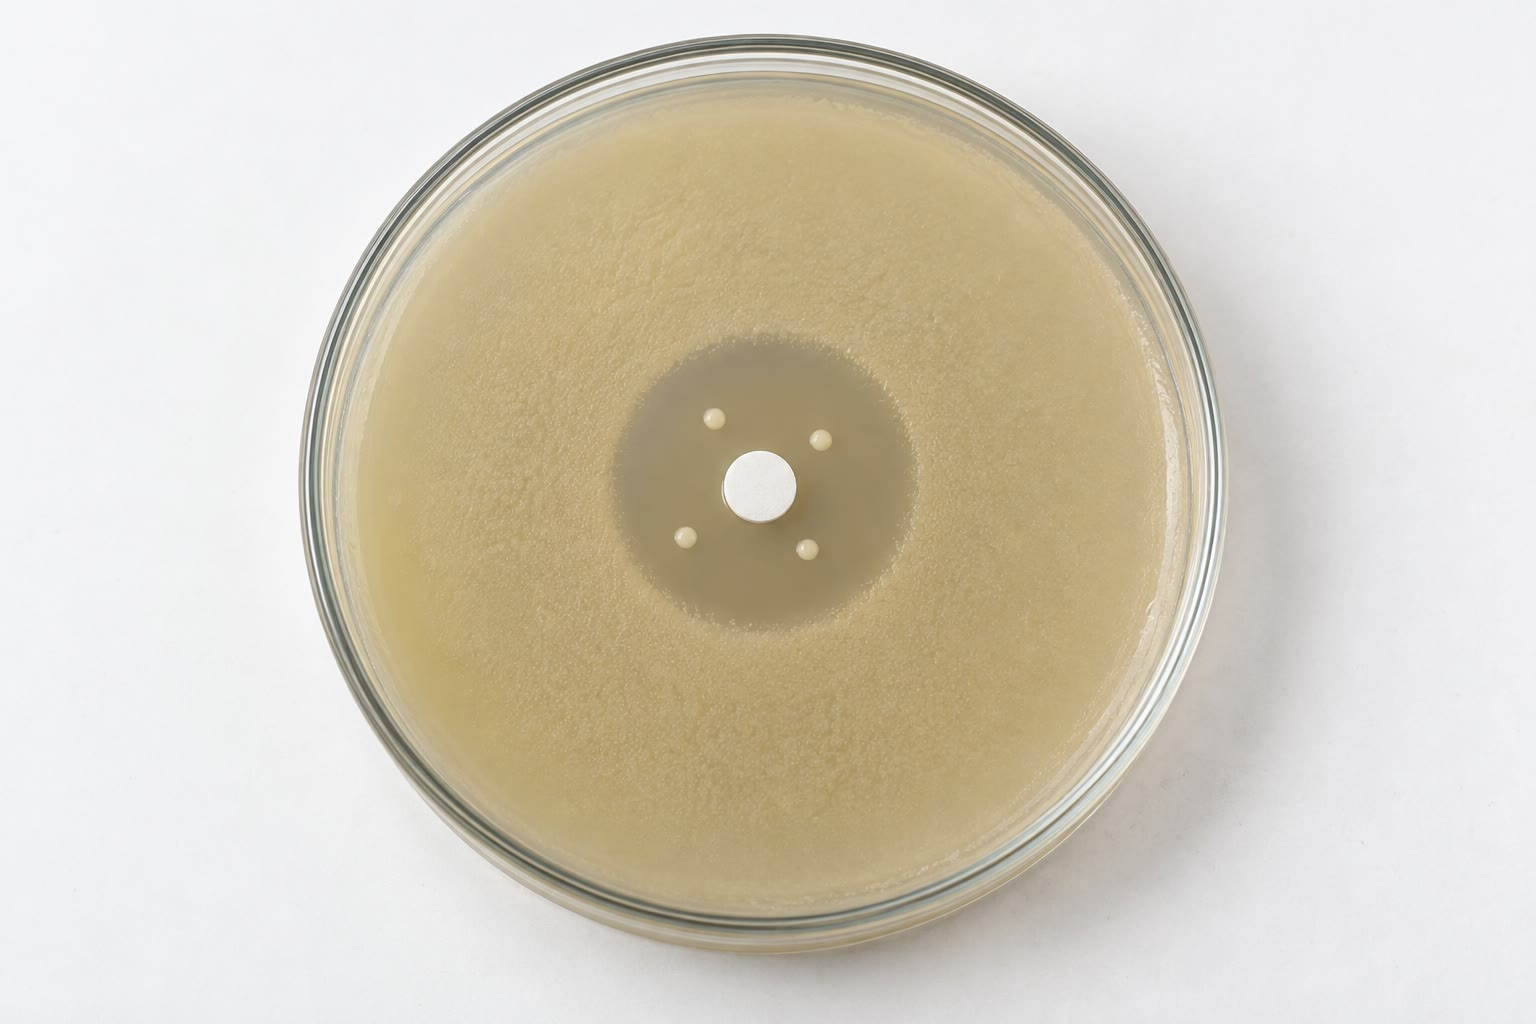
\includegraphics[width=0.5\linewidth]{images/book4/ai/b4-03-luria-plate.jpg}

{\small Een antibioticumschijfje op een bacteriegazon: de heldere zone is
waar het middel dat uit het schijfje diffundeert de gevoelige cellen
heeft gedood, en de kolonies daarbinnen zijn gegroeid uit resistente
mutanten die al aanwezig waren voordat het schijfje werd neergelegd.}
\end{omfigure}

\begin{proposition}[Herstel en zijn grenzen]\label{prop:b2:genome-diversification:repair}
\index{DNA-herstel}
Een cel corrigeert de meeste schade voordat die een \omterm{def:b2:genome-diversification:mutation}{mutatie} wordt.
\emph{Mismatchherstel} verwijdert de verkeerde base uit de nieuw
gemaakte streng. \emph{Base-excisieherstel} knipt één beschadigde base
weg (een uracil, een geoxideerd guanine) en vult het gat op; het is de
reden waarom DNA thymine gebruikt in plaats van uracil: een uracil in
DNA kan alleen een gedeamineerd cytosine zijn, en wordt als vreemd
herkend. \emph{Nucleotide-excisieherstel} verwijdert een stuk van een
twaalftal basen rond een omvangrijke beschadiging zoals een
thyminedimeer; mensen bij wie het ontbreekt (xeroderma pigmentosum),
krijgen huidkanker door gewoon zonlicht.
\emph{Recombinatieherstel} bouwt een gebroken chromosoom opnieuw op aan
de hand van de zusterkopie. Wat aan herstel ontsnapt, of verkeerd wordt
hersteld, is een \omterm{def:b2:genome-diversification:mutation}{mutatie} --- en een cel die een herstelsysteem heeft
verloren (een \emph{mutator}), muteert honderd keer sneller, wat op
korte termijn een voordeel is onder stress en op lange termijn een last.
Herstelmechanismen worden uitgebreid behandeld in het deel van jaar 3.
\end{proposition}

\section{Genen die bewegen}

\begin{definition}[Transponeerbare elementen]\label{def:b2:genome-diversification:transposon}
\index{transposon}\index{retrotransposon}
Een \emph{transponeerbaar element} is een DNA-segment dat zich naar een
nieuwe positie in het genoom kan verplaatsen. \emph{DNA-transposons}
coderen voor een \emph{transposase} die het element uitknipt en elders
inplakt (of het daar kopieert); bacteriële insertiesequenties zijn de
eenvoudigste (een transposasegen tussen twee omgekeerde herhalingen), en
samengestelde transposons dragen tussen twee daarvan extra genen ---
vaak antibioticumresistenties. \emph{Retrotransposons} verplaatsen zich
langs een kopiëren-en-plakkenroute via een RNA-tussenproduct, dat door
een reverse transcriptase weer in DNA wordt omgeschreven; ze verlaten
hun oude plaats nooit en hopen zich dus op. Een element dat in een gen
belandt, verstoort het; belandt het ernaast, dan kan het de expressie
ervan veranderen; twee kopieën in één chromosoom bieden plaatsen voor
\omterm{prop:b2:genome-diversification:duplication}{ongelijke crossing-over}. Transposons en hun overblijfselen vormen de
helft van het menselijke genoom en tachtig procent van het genoom van
maïs; de meeste zijn nu onbeweeglijk.
\end{definition}
\begin{proof}[Bewijsmateriaal]
McClintock (jaren 1940--1950) bestudeerde maïskorrels waarvan het paarse
pigment in sommige cellen verloren ging en in andere werd hersteld, wat
gespikkelde korrels gaf. Ze toonde door kruisingen en door
chromosoomwaarnemingen aan dat de instabiliteit werd veroorzaakt door
een element (\emph{Dissociation}) dat het chromosoom brak waar het zat
en tussen posities bewoog onder controle van een tweede element
(\emph{Activator}), en dat een gen werd uitgeschakeld wanneer het
element erin zat en weer werd geactiveerd wanneer het vertrok. Genen,
concludeerde ze, konden van positie veranderen; het idee werd pas
twintig jaar later aanvaard, toen bacteriële insertiesequenties werden
gevonden, en leverde haar in 1983 een Nobelprijs op.
\end{proof}

\begin{omfigure}
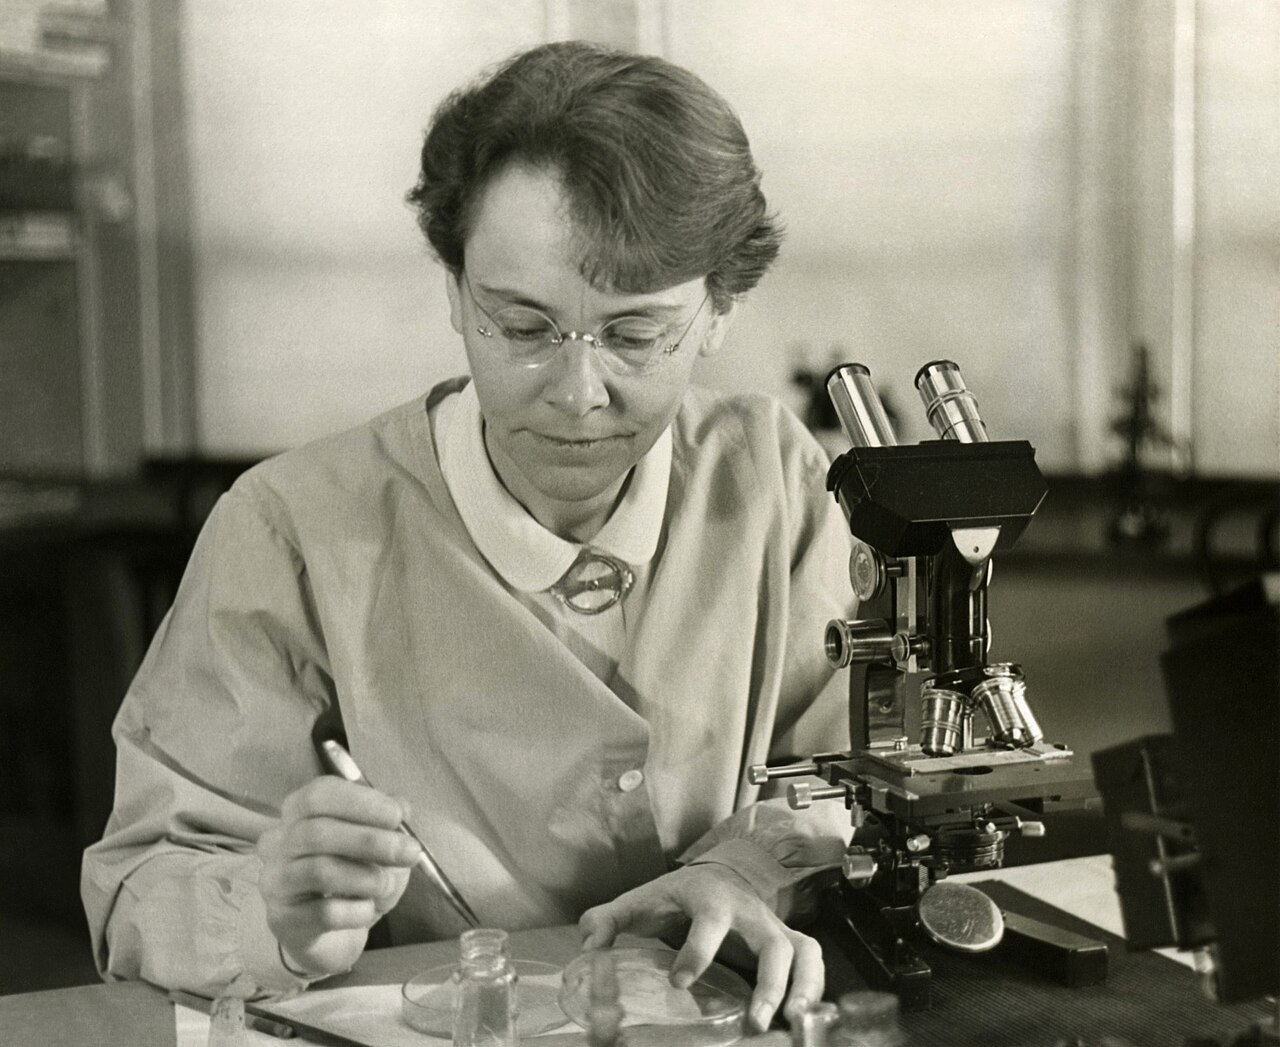
\includegraphics[width=0.4\linewidth]{images/book4/mcclintock.jpg}\hspace{0.04\linewidth}
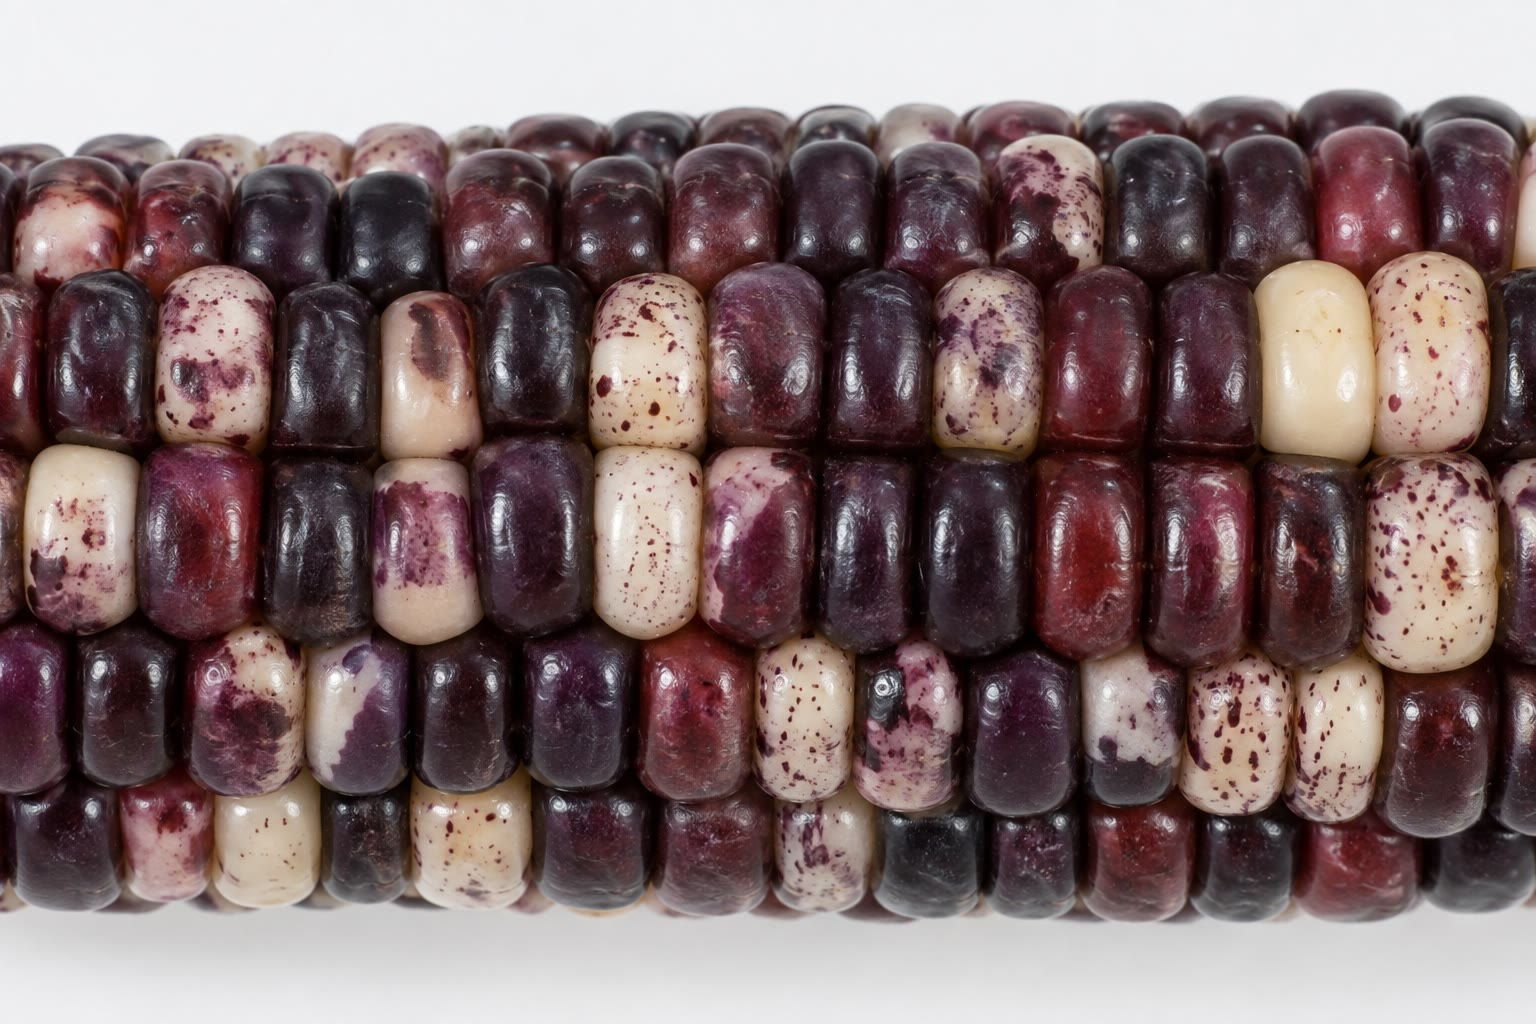
\includegraphics[width=0.5\linewidth]{images/book4/ai/b4-03-maize-kernels.jpg}

{\small Barbara McClintock, en de korrels die haar naar transponeerbare
elementen leidden: een gen voor paars pigment dat door een ingevoegd
element wordt uitgeschakeld en cel voor cel weer wordt aangeschakeld
wanneer het element eruit springt, wat spikkels en sectoren achterlaat.}
\end{omfigure}

\begin{omfigure}
\begin{tikzpicture}[every node/.style={font=\scriptsize}]
  % cut and paste
  \begin{scope}
    \draw[very thick, gray] (0,1.2) -- (4.5,1.2);
    \fill[omThm!70] (0.8,1.05) rectangle (1.8,1.35); \node[white, font=\tiny] at (1.3,1.2) {Tn};
    \draw[very thick, gray] (0,0) -- (4.5,0);
    \fill[omThm!70] (2.8,-0.15) rectangle (3.8,0.15); \node[white, font=\tiny] at (3.3,0) {Tn};
    \draw[->, thick, omThm] (1.3,1.0) .. controls (1.3,0.5) and (3.3,0.7) .. (3.3,0.2);
    \draw[dashed, gray] (0.8,1.2) -- (1.8,1.2);
    \node[align=center] at (2.25,-0.6) {knippen en plakken (DNA-transposon):\\het element verlaat zijn oude plaats};
  \end{scope}
  % copy and paste
  \begin{scope}[xshift=7.5cm]
    \draw[very thick, gray] (0,1.2) -- (4.5,1.2);
    \fill[omProp!80] (0.8,1.05) rectangle (1.8,1.35); \node[white, font=\tiny] at (1.3,1.2) {RT};
    \draw[very thick, gray] (0,0) -- (4.5,0);
    \fill[omProp!80] (2.8,-0.15) rectangle (3.8,0.15); \node[white, font=\tiny] at (3.3,0) {RT};
    \draw[->, thick, omProp] (1.3,1.0) .. controls (1.3,0.5) and (3.3,0.7) .. (3.3,0.2);
    \node[omProp, anchor=west, align=left] at (3.6,0.75) {RNA-kopie,\\omgekeerd getranscribeerd};
    \node[align=center] at (2.25,-0.6) {kopiëren en plakken (retrotransposon):\\de oude kopie blijft, het aantal groeit};
  \end{scope}
\end{tikzpicture}

{\small Twee manieren om te bewegen. Een \omterm{def:b2:genome-diversification:transposon}{DNA-transposon} wordt uitgeknipt
en opnieuw ingevoegd; een \omterm{def:b2:genome-diversification:transposon}{retrotransposon} wordt getranscribeerd, weer in
DNA gekopieerd en elders ingevoegd, zodat zijn kopieën zich ophopen.}
\end{omfigure}

\begin{definition}[Horizontale genoverdracht]\label{def:b2:genome-diversification:hgt}
\index{horizontale genoverdracht}\index{transformatie}\index{conjugatie!bacteriële}\index{transductie}
Prokaryoten verwerven langs drie routes genen van cellen die niet hun
ouders zijn. \emph{Transformatie}: een cel neemt naakt DNA op uit haar
omgeving (vrijgekomen uit dode cellen) en recombineert het in haar
chromosoom; sommige soorten zijn van nature competent, en langs deze
route wisselen pneumokokken kapselgenen uit. \emph{Conjugatie}: een
donor met een conjugatief \omterm{def:b2:unicellular-diversity:prokaryote}{plasmide} (de F-factor van \emph{E.~coli})
bouwt een pilus, trekt een ontvanger dichtbij en voert één streng van
het \omterm{def:b2:unicellular-diversity:prokaryote}{plasmide} door een porie, terwijl hij het volgens de rollende cirkel
repliceert; als het \omterm{def:b2:unicellular-diversity:prokaryote}{plasmide} in het chromosoom is geïntegreerd (een
Hfr-stam), worden chromosomale genen in volgorde erachter overgedragen,
en het moment waarop elk gen binnenkomt, brengt het chromosoom in kaart.
\emph{Transductie}: een bacteriofaag verpakt per vergissing een stuk
gastheer-DNA en injecteert het in de volgende cel die hij infecteert.
Samen verplaatsen deze routes resistentiegenen binnen enkele jaren
tussen soorten in ziekenhuizen, en hebben ze over geologische tijd
metabole genen over de hele bacteriële boom verplaatst, zodat de afstamming
van een \omterm{def:b2:unicellular-diversity:prokaryote}{prokaryoot} evengoed een web als een boom is
(\cref{ch:b2:phylogenetic-trees}).
\end{definition}
\begin{proof}[Bewijsmateriaal]
Lederberg en Tatum (1946) mengden twee stammen van \emph{E.~coli}, die
elk twee verschillende voedingsstoffen niet konden maken, en plaatten het
mengsel uit op een minimaal medium waarop geen van beide alleen kon
groeien: er verschenen kolonies, ongeveer één per tien miljoen cellen,
die alle vier konden maken --- recombinanten. Davis (1950) herhaalde het
met de stammen gescheiden door een filter dat moleculen doorliet maar
geen cellen: geen recombinanten, dus was contact nodig. Hayes toonde
vervolgens aan dat de overdracht in één richting verliep, van een donor
naar een ontvanger, en Wollman en Jacob (1956) onderbraken paringen met
tussenpozen in een blender en vonden dat de genen van de donor in een
vaste volgorde de ontvanger binnenkwamen, het ene na het andere, over
ongeveer honderd minuten.
\end{proof}

\begin{omfigure}
\begin{minipage}[b]{0.56\linewidth}\centering
\begin{tikzpicture}[every node/.style={font=\scriptsize}]
  % donor
  \draw[thick, fill=omDef!8] (0,0) ellipse (1.5 and 0.75);
  \draw[thick, omDef] (0.2,0) circle (0.45);
  \draw[thick, omThm] (-0.9,0.1) circle (0.22);
  \node[anchor=south] at (0,1.25) {donor $F^+$};
  \draw[omThm] (-0.9,-0.12) -- (-1.1,-1.0) node[below] {F-plasmide};
  \draw[omDef] (0.4,-0.4) -- (0.6,-1.0) node[below] {chromosoom};
  % recipient
  \draw[thick, fill=omDef!8] (5,0) ellipse (1.5 and 0.75);
  \draw[thick, omDef] (5.2,0) circle (0.45);
  \node[anchor=south] at (5,1.25) {ontvanger $F^-$};
  % pilus
  \draw[very thick, omThm] (1.5,0) -- (3.5,0);
  \node[omThm, below] at (2.5,-0.05) {pilus};
  % single strand transferred
  \draw[->, thick, omThm, dashed] (-0.7,0.15) .. controls (1.0,0.7) and (3.0,0.7) .. (4.1,0.4);
  \node[omThm, anchor=south] at (2.5,0.7) {één streng gekopieerd via rollende cirkel};
  \draw[thick, omThm, dashed] (4.1,0.2) circle (0.2);
\end{tikzpicture}
\end{minipage}\hfill
\begin{minipage}[b]{0.42\linewidth}\centering
\begin{tikzpicture}
\begin{axis}[
  width=\linewidth, height=4.6cm,
  axis x line=bottom, axis y line=left,
  xmin=0, xmax=40, ymin=0, ymax=1.1,
  xlabel={minuten vóór het mixen}, ylabel={recombinanten (relatief)},
  xlabel style={font=\scriptsize, at={(axis description cs:0.5,-0.18)}, anchor=north},
  ylabel style={font=\scriptsize},
  tick label style={font=\scriptsize}, xtick={0,10,20,30,40}, ytick={0,0.5,1},
  legend style={font=\scriptsize, at={(0.97,0.08)}, anchor=south east, draw=none},
  clip=false,
]
\addplot[very thick, omDef, domain=8:40, samples=40] {1-exp(-(x-8)/5)};
\addlegendentry{\emph{thr}, komt binnen na \qty{8}{min}}
\addplot[very thick, omProp, domain=17:40, samples=40] {1-exp(-(x-17)/5)};
\addlegendentry{\emph{lac}, \qty{17}{min}}
\addplot[very thick, omThm, domain=25:40, samples=40] {1-exp(-(x-25)/5)};
\addlegendentry{\emph{gal}, \qty{25}{min}}
\end{axis}
\end{tikzpicture}
\end{minipage}

{\small Links: conjugatie --- de donor voert één streng van zijn
\omterm{def:b2:unicellular-diversity:prokaryote}{F-plasmide} door de verbinding van de pilus terwijl hij die kopieert.
Rechts: het experiment met onderbroken paring met een Hfr-donor: elk
chromosomaal gen verschijnt op een kenmerkend tijdstip onder de
recombinanten, wat het chromosoom in minuten in kaart brengt.}
\end{omfigure}

\begin{omfigure}
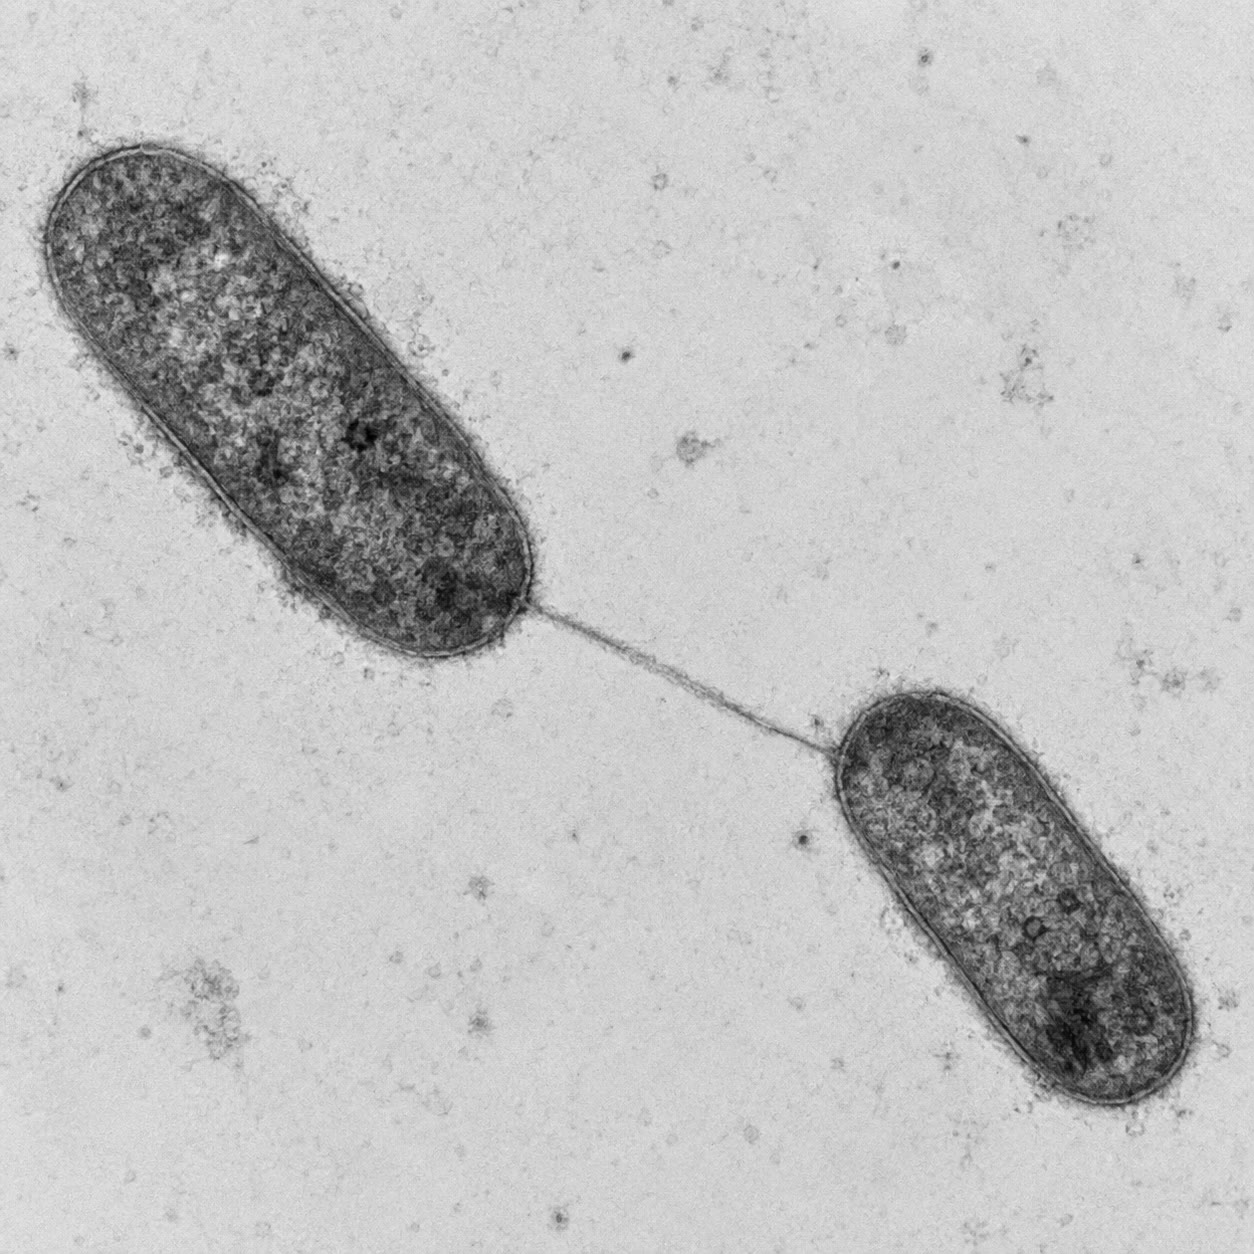
\includegraphics[width=0.42\linewidth]{images/book4/ai/b4-03-conjugation-tem.jpg}

{\small Twee bacteriën verbonden door een conjugatieve pilus, gezien met
de transmissie-elektronenmicroscoop: de brug waarlangs het \omterm{def:b2:unicellular-diversity:prokaryote}{plasmide}
passeert.}
\end{omfigure}

\begin{example}[Resistentie op reis]\label{ex:b2:genome-diversification:resistance}
Een resistentiegen ontstaat doorgaans één keer, door \omterm{def:b2:genome-diversification:mutation}{mutatie} of vanuit
de bodembacterie die het antibioticum maakt, en gaat dan op reis: van
een chromosoom naar een \omterm{def:b2:genome-diversification:transposon}{transposon}, van het \omterm{def:b2:genome-diversification:transposon}{transposon} naar een
conjugatief \omterm{def:b2:unicellular-diversity:prokaryote}{plasmide}, van het \omterm{def:b2:unicellular-diversity:prokaryote}{plasmide} via conjugatie naar andere soorten
en via \omterm{def:b2:genome-diversification:hgt}{transductie} naar andere stammen, en via \omterm{def:b2:genome-diversification:hgt}{transformatie} terug in
een chromosoom. \omterm{def:b2:unicellular-diversity:prokaryote}{Plasmiden} met vijf of zes resistenties tegelijk
(samengebracht in \emph{integronen}, die gencassettes invangen) werden in
de jaren 1950 in Japan gevonden, enkele jaren nadat de middelen in
gebruik kwamen; het gen voor het carbapenemase NDM-1, voor het eerst
gezien in 2008, bereikte binnen drie jaar op een \omterm{def:b2:unicellular-diversity:prokaryote}{plasmide} elk continent.
De evolutie van resistentie is meestal niet de evolutie van nieuwe genen,
maar de verplaatsing van oude.
\end{example}

\section{Duplicatie: genen en genomen}

\begin{proposition}[Genduplicatie en genfamilies]\label{prop:b2:genome-diversification:duplication}
\index{genduplicatie}\index{genfamilie}\index{ongelijke crossing-over}
Wanneer twee gelijkende sequenties achter elkaar op een chromosoom
liggen, kunnen de homologen bij de meiose verschoven paren en ongelijk
overkruisen, zodat het ene product drie kopieën draagt en het andere
één. Een gedupliceerd gen is overbodig: de ene kopie kan de oude taak
blijven vervullen terwijl de andere vrij \omterm{def:b2:genome-diversification:mutation}{mutaties} opstapelt --- meestal
vervalt die tot een \emph{pseudogen}, soms verwerft ze een nieuwe functie
(\emph{neofunctionalisatie}) of een deel van de oude
(\emph{subfunctionalisatie}). Herhaald over honderden miljoenen jaren
bouwt dit \emph{genfamilies} op: de globines (één voorouderlijk gen werd
myoglobine, de $\alpha$-cluster en de $\beta$-cluster, met embryonale,
foetale en volwassen leden die na elkaar tot expressie komen), de
geurreceptoren (duizend genen bij een muis), de homeoboxgenen, de
kristallines van de lens. De meeste genen van een genoom behoren tot een
familie, en duplicatie is de belangrijkste bron van nieuwe genen.
\end{proposition}
\begin{proof}[Bewijsmateriaal]
De menselijke $\beta$-globinecluster op chromosoom 11 bevat vijf
functionele genen ($\varepsilon$, $^{G}\gamma$, $^{A}\gamma$,
$\delta$, $\beta$) en een pseudogen, in de volgorde waarin ze tijdens
de ontwikkeling worden aangeschakeld, alle met dezelfde exon-intronstructuur,
en met sequenties die meer op elkaar lijken naarmate ze recenter zijn
uiteengegaan; de $\alpha$-cluster op chromosoom 16 heeft dezelfde
architectuur. Deleties van één of meer $\alpha$-genen, ontstaan door
\omterm{prop:b2:genome-diversification:duplication}{ongelijke crossing-over} tussen de bijna identieke kopieën, komen vaak
voor en veroorzaken $\alpha$-thalassemie; het wederkerige product, een
chromosoom met drie $\alpha$-genen, wordt in dezelfde populaties
aangetroffen.
\end{proof}

\begin{omfigure}
\begin{tikzpicture}[every node/.style={font=\scriptsize}]
  % unequal crossing over
  \begin{scope}
    \draw[very thick, gray] (0,1.2) -- (5,1.2);
    \fill[omDef!70] (1.0,1.05) rectangle (2.0,1.35); \fill[omDef!70] (2.4,1.05) rectangle (3.4,1.35);
    \draw[very thick, gray] (0,0) -- (5,0);
    \fill[omDef!70] (1.0,-0.15) rectangle (2.0,0.15); \fill[omDef!70] (2.4,-0.15) rectangle (3.4,0.15);
    \node[above] at (1.5,1.35) {A}; \node[above] at (2.9,1.35) {A$'$};
    \draw[very thick, omThm] (2.9,1.05) -- (1.5,0.15);
    \node[align=center] at (2.5,-0.6) {verschoven gepaarde homologen\\kruisen ongelijk over};
    \draw[->, thick, gray] (5.3,0.6) -- (6.1,0.6);
    % products
    \draw[very thick, gray] (6.5,1.2) -- (11.5,1.2);
    \fill[omDef!70] (7.5,1.05) rectangle (8.5,1.35); \fill[omDef!70] (8.9,1.05) rectangle (9.9,1.35); \fill[omDef!70] (10.3,1.05) rectangle (11.3,1.35);
    \node[above] at (9.4,1.35) {drie kopieën};
    \draw[very thick, gray] (6.5,0) -- (11.5,0);
    \fill[omDef!70] (7.5,-0.15) rectangle (8.5,0.15);
    \node[above] at (8.0,0.15) {één kopie};
  \end{scope}
  % globin family tree
  \begin{scope}[yshift=-3.6cm]
    \draw[thick] (2,2.2) -- (2,1.7);
    \draw[thick] (0.5,1.7) -- (3.5,1.7);
    \draw[thick] (0.5,1.7) -- (0.5,0.4); \node[below] at (0.5,0.4) {myoglobine};
    \draw[thick] (3.5,1.7) -- (3.5,1.2);
    \draw[thick] (2.3,1.2) -- (4.7,1.2);
    \draw[thick] (2.3,1.2) -- (2.3,0.4); \node[below] at (2.3,0.4) {$\alpha$-familie};
    \draw[thick] (4.7,1.2) -- (4.7,0.9);
    \draw[thick] (3.6,0.9) -- (5.8,0.9);
    \draw[thick] (3.6,0.9) -- (3.6,0.4); \node[below] at (3.6,0.4) {$\varepsilon,\gamma$};
    \draw[thick] (5.8,0.9) -- (5.8,0.7);
    \draw[thick] (5.2,0.7) -- (6.4,0.7);
    \draw[thick] (5.2,0.7) -- (5.2,0.4); \node[below] at (5.2,0.4) {$\delta$};
    \draw[thick] (6.4,0.7) -- (6.4,0.4); \node[below] at (6.4,0.4) {$\beta$};
    \node[anchor=west, align=left] at (7.2,1.7) {duplicaties van één voorouderlijk globinegen:\\vóór de gewervelden (myoglobine/hemoglobine),\\$\sim$450 miljoen jaar geleden ($\alpha$/$\beta$),\\daarna binnen de $\beta$-cluster (embryonaal, foetaal, volwassen)};
    \node[anchor=east, gray] at (1.9,2.1) {voorouderlijk globine};
  \end{scope}
\end{tikzpicture}

{\small Boven: \omterm{prop:b2:genome-diversification:duplication}{ongelijke crossing-over} tussen verschoven gepaarde
tandemkopieën levert een chromosoom met drie kopieën en een met één
kopie. Onder: de globinefamilie, opgebouwd door opeenvolgende duplicaties
en divergentie.}
\end{omfigure}

\begin{definition}[Polyploïdie]\label{def:b2:genome-diversification:polyploidy}
\index{polyploïdie}\index{allopolyploïd}\index{autopolyploïd}
Een \emph{polyploïd} draagt meer dan twee volledige chromosoomsets.
Een \emph{autopolyploïd} heeft meerdere sets van één soort (een mislukte
meiose geeft een diploïde gameet; twee zulke gameten geven een
tetraploïd); een \emph{allopolyploïd} combineert de sets van twee
soorten na een hybridisatie. De diploïde hybride AB, zonder homoloog voor
welk chromosoom ook, kan ze bij de meiose niet paren en is steriel;
verdubbelt haar genoom tot AABB, dan heeft elk chromosoom weer een
partner, werkt de meiose, en is de nieuwe plant vruchtbaar --- maar kan
ze niet terugkruisen met een van beide ouders (een nakomeling AAB is
steriel). Polyploïdie maakt zo in één stap een nieuwe soort, en ongeveer
een derde van de soorten bloemplanten is zo ontstaan: broodtarwe is een
hexaploïde AABBDD van drie grassen, de tuinaardbei een octoploïde,
katoen en tabak zijn allotetraploïden, en de lijn van de gewervelden
heeft zelf nabij haar oorsprong tweemaal haar genoom verdubbeld.
Polyploïden zijn meestal groter dan hun diploïde voorouders (meer DNA,
grotere cellen) en zeer gewild bij veredelaars.
\end{definition}

\begin{omfigure}
\begin{tikzpicture}[every node/.style={font=\scriptsize}]
  \node[draw, rounded corners, fill=omDef!10, align=center] (a) at (0,0) {\emph{T.~urartu}\\AA, $2n = 14$};
  \node[draw, rounded corners, fill=omDef!10, align=center] (b) at (3.4,0) {\emph{Aegilops}\\BB, $2n = 14$};
  \node[draw, rounded corners, fill=omProp!15, align=center] (ab) at (1.7,-1.5) {hybride AB\\$n = 14$, steriel};
  \node[draw, rounded corners, fill=omExo!25, align=center] (aabb) at (1.7,-3.1) {emmertarwe AABB\\$2n = 28$, vruchtbaar};
  \node[draw, rounded corners, fill=omDef!10, align=center] (d) at (6.4,-3.1) {\emph{Ae.~tauschii}\\DD, $2n = 14$};
  \node[draw, rounded corners, fill=omProp!15, align=center] (abd) at (4.0,-4.6) {hybride ABD\\$3n = 21$, steriel};
  \node[draw, rounded corners, fill=omExo!25, align=center] (abd2) at (4.0,-6.1) {broodtarwe AABBDD\\$2n = 42$, vruchtbaar};
  \draw[->, thick] (a) -- (ab); \draw[->, thick] (b) -- (ab);
  \draw[->, thick] (ab) -- (aabb) node[midway, right] {genoomverdubbeling};
  \draw[->, thick] (aabb) -- (abd); \draw[->, thick] (d) -- (abd);
  \draw[->, thick] (abd) -- (abd2) node[midway, right] {genoomverdubbeling};
  \node[anchor=west, align=left, gray] at (7.8,-1.5) {elke hybridisatie geeft een steriele\\plant met ongepaarde chromosomen;\\elke verdubbeling herstelt de paring\\en de vruchtbaarheid --- en maakt een\\soort die niet kan terugkruisen};
\end{tikzpicture}

{\small De oorsprong van broodtarwe: twee hybridisaties, elk gevolgd door
een verdubbeling van het genoom, bouwden in ongeveer tienduizend jaar
een hexaploïde uit drie diploïde grassen.}
\end{omfigure}

\begin{omfigure}
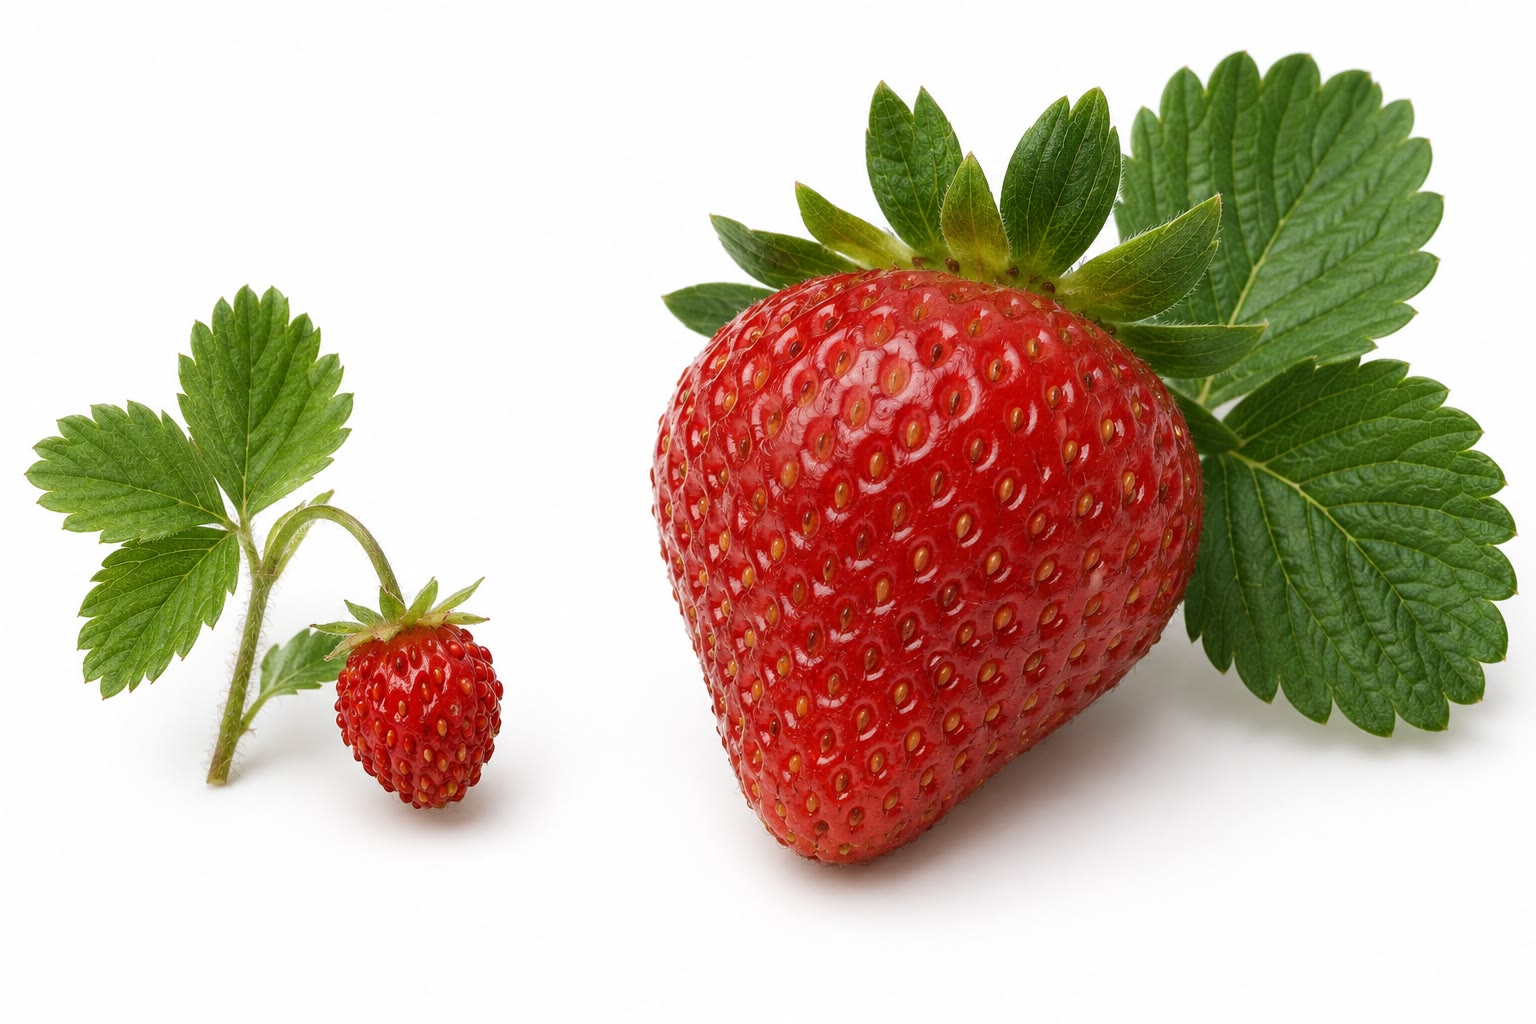
\includegraphics[width=0.55\linewidth]{images/book4/ai/b4-03-polyploid-strawberries.jpg}

{\small Een wilde diploïde aardbei en de gekweekte octoploïde: de
polyploïde, met vier keer zoveel DNA in elke cel, is de grotere plant
met de grotere vrucht.}
\end{omfigure}

\section{Toeval en snelheid}

\begin{proposition}[Mutatie is willekeurig ten opzichte van de behoefte]\label{prop:b2:genome-diversification:random}
\index{mutatie!willekeurigheid van}
De \omterm{thm:b2:genome-diversification:luria}{fluctuatietest} en het replicaplaten tonen aan dat een \omterm{def:b2:genome-diversification:mutation}{mutatie} die in
een nieuwe omgeving nuttig is, met dezelfde snelheid ontstaat of die
omgeving nu aanwezig is of niet: de omgeving selecteert tussen \omterm{def:b2:genome-diversification:mutation}{mutaties},
ze roept ze niet op. \omterm{def:b2:genome-diversification:mutation}{Mutatie} is niet in elke zin willekeurig ---
transities zijn talrijker dan transversies, CpG-dinucleotiden muteren tien
keer sneller dan andere plaatsen (hun gemethyleerde cytosine deamineert
tot thymine, dat het herstel niet als vreemd herkent), sommige gebieden
zijn hotspots, en stress kan de algehele snelheid verhogen --- maar ze
is blind voor de gevolgen. De \omterm{thm:b2:genome-diversification:rate}{mutatiesnelheid} zelf is een erfelijke
eigenschap, en selectie stelt haar bij: te hoog, en elke generatie erft
schadelijke veranderingen; te laag, en de populatie kan een veranderende
wereld niet volgen. Mutatorstammen winnen kortstondig in een ziekenhuis
en verliezen op den duur, en de snelheid van $10^{-9}$ per base waarop
de meeste cellen uitkomen, is een compromis tussen de kosten van fouten
en de kosten van proeflezen.
\end{proposition}

\section{Opgaven}

\begin{exercise}[$\star$]\label{exo:b2:genome-diversification:1}
Deel elke verandering van het codon GAA (glutamaat) in: GAG; GTA; TAA;
insertie van een C na de eerste base. Welke is een transitie, welke een
transversie?
\end{exercise}

\begin{exercise}[$\star$]\label{exo:b2:genome-diversification:2}
Met $u = \qty{5e-10}{}$ per basenpaar per replicatie en $G =
\qty{4.6e6}{}$: hoeveel nieuwe \omterm{def:b2:genome-diversification:mutation}{mutaties} levert één deling van
\emph{E.~coli} gemiddeld op? Hoeveel per generatie in een cultuur van
$10^{9}$ cellen?
\end{exercise}

\begin{exercise}[$\star$]\label{exo:b2:genome-diversification:3}
Noem de drie routes van \omterm{def:b2:genome-diversification:hgt}{horizontale genoverdracht} en zeg bij elk wat ze
vereist (contact, een virus, vrij DNA) en wat ze doorgaans overdraagt.
\end{exercise}

\begin{exercise}[$\star$]\label{exo:b2:genome-diversification:4}
Onderscheid autopolyploïdie van allopolyploïdie, met een voorbeeld van
elk, en leg uit waarom een diploïde hybride van twee soorten meestal
steriel is.
\end{exercise}

\begin{exercise}[$\star\star$]\label{exo:b2:genome-diversification:5}
Een menselijke kiembaan stapelt $u = \qty{1.2e-8}{}$ \omterm{def:b2:genome-diversification:mutation}{mutaties} per
basenpaar per generatie op over een haploïd genoom van \qty{3.2e9}{}
basenparen. Hoeveel nieuwe \omterm{def:b2:genome-diversification:mutation}{mutaties} draagt een kind? Als \qty{1.5}{\%}
van het genoom voor eiwit codeert en \qty{70}{\%} van de coderende
substituties een aminozuur verandert, hoeveel nieuwe aminozuurveranderingen
draagt het kind dan?
\end{exercise}

\begin{exercise}[$\star\star$]\label{exo:b2:genome-diversification:6}
Een cultuur groeit van $10^{3}$ tot $10^{9}$ cellen; een bepaalde \omterm{def:b2:genome-diversification:mutation}{mutatie}
treedt op met $m = \qty{2e-8}{}$ per deling. Bereken het verwachte aantal
mutatiegebeurtenissen en mutante cellen. Waarom is de fractie culturen
zonder mutant hier onbruikbaar om $m$ te meten, en welke grootte van de
cultuur zou haar bruikbaar maken?
\end{exercise}

\begin{exercise}[$\star\star$]\label{exo:b2:genome-diversification:7}
Cytosine deamineert tot uracil; 5-methylcytosine deamineert tot thymine.
Leg uit waarom het eerste efficiënt wordt hersteld en het tweede niet,
en leid af waarom CpG-plaatsen (waar cytosine gemethyleerd is)
mutatiehotspots zijn en zeldzamer in het genoom dan het toeval zou
voorspellen.
\end{exercise}

\begin{exercise}[$\star\star$]\label{exo:b2:genome-diversification:8}
In een experiment met onderbroken paring komen vier genen de ontvanger
binnen na 8, 17, 25 en \qty{40}{min}; het hele chromosoom (\qty{4.6}{Mb})
zou \qty{100}{min} vergen. Zet de tijden om in posities in kilobasen en
bereken de afstanden tussen opeenvolgende genen.
\end{exercise}

\begin{exercise}[$\star\star$]\label{exo:b2:genome-diversification:9}
Teken de paring en de crossing-over die van twee chromosomen met elk twee
tandemgenen voor $\alpha$-globine er één met drie en één met één maken.
Iemand erft van elke ouder een chromosoom met één gen: hoeveel
$\alpha$-genen heeft die persoon, en wat valt er van zijn hemoglobine te
verwachten?
\end{exercise}

\begin{exercise}[$\star\star\star$]\label{exo:b2:genome-diversification:10}
Broodtarwe is AABBDD met $2n = 42$. Geef het chromosoomaantal van haar
gameten, van de steriele hybriden bij elke stap van haar ontstaan, en van
een kruising tussen broodtarwe en emmertarwe (AABB). Leg in termen van
meiotische paring uit waarom elke verdubbeling de vruchtbaarheid
herstelde en waarom de hexaploïde niet met haar ouders kan terugkruisen.
\end{exercise}

\begin{exercise}[$\star\star\star$]\label{exo:b2:genome-diversification:11}
In een darmpopulatie van $N = 10^{9}$ bacteriën verspreidt een
resistentieplasmide zich via conjugatie met een snelheid die evenredig is
met de ontmoetingen tussen dragers $R$ en niet-dragers $N - R$: $\mathrm{d}R/\mathrm{d}t =
\gamma R (N - R)$ met $\gamma N = \qty{0.5}{h^{-1}}$. Los op, uitgaande van één drager, en
bereken de tijd tot de helft van de populatie het \omterm{def:b2:unicellular-diversity:prokaryote}{plasmide} draagt. Wat
gebeurt er als het antibioticum daarna wordt stopgezet en het \omterm{def:b2:unicellular-diversity:prokaryote}{plasmide}
zijn gastheer \qty{5}{\%} aan groeisnelheid kost?
\end{exercise}

\begin{exercise}[$\star\star\star$]\label{exo:b2:genome-diversification:12}
``\omterm{def:b2:genome-diversification:mutation}{Mutatie} is willekeurig; evolutie niet.'' Bespreek dit aan de hand van
de \omterm{thm:b2:genome-diversification:luria}{fluctuatietest}, het replicaplaten en het feit dat de \omterm{thm:b2:genome-diversification:rate}{mutatiesnelheid}
zelf aan selectie onderhevig is.
\end{exercise}

\section{Vraagstuk: een fluctuatietest}

\begin{problem}[{Weekendvraagstuk --- een fluctuatietest wordt uitgevoerd
en geanalyseerd, de mutatiesnelheid van een stam eruit afgeleid en
opgeschaald naar haar genoom en haar populatie, de verspreiding van een
resistentieplasmide gemodelleerd en de kosten van een mutator gewogen,
met als besluit de mutatiesnelheid van de stam per base en de tijd die
het plasmide nodig heeft om de overhand te krijgen}]
\label{pb:b2:genome-diversification:1}
Twintig culturen van \emph{E.~coli} worden elk gestart met \num{100}
cellen in \qty{0.2}{mL} en gekweekt tot $N = \qty{2e8}{}$ cellen; elke
cultuur wordt dan uitgestreken op een plaat met een bacteriofaag, en de
resistente kolonies worden geteld: 0, 0, 0, 1, 0, 0, 3, 0, 0, 1, 0, 0,
0, 0, 107, 0, 2, 0, 0, 5. Tegelijk worden twintig monsters van
\qty{0.2}{mL} genomen uit één grote cultuur met dezelfde dichtheid en op
dezelfde manier uitgeplaat: 14, 15, 13, 21, 15, 14, 26, 16, 20, 13, 17,
12, 18, 14, 16, 19, 15, 13, 17, 16. Genoom: \qty{4.6e6}{} basenparen,
\qty{88}{\%} coderend. Resistentie tegen de faag kan ontstaan door elk
van \num{20} verschillende veranderingen van één base in één receptorgen.

\medskip
\noindent\textbf{Deel I --- De test.}
\begin{enumerate}
  \item Bereken het gemiddelde en de variantie van de twintig
        onafhankelijke culturen.
  \item Bereken het gemiddelde en de variantie van de twintig monsters.
  \item Bij een poissonverdeling is de variantie gelijk aan het
        gemiddelde. Welke reeks is poissonverdeeld, en wat zegt de
        verdeling van elke reeks over \emph{wanneer} de \omterm{def:b2:genome-diversification:mutation}{mutaties} optraden?
  \item Verklaar het aantal van 107.
  \item Hoeveel van de onafhankelijke culturen bevatten geen mutant? Gebruik
        $p_0 = e^{-m(N - N_0)}$ om $m$ te schatten, de \omterm{thm:b2:genome-diversification:rate}{mutatiesnelheid} naar
        resistentie per celdeling.
  \item Bereken het verwachte aantal mutante cellen per cultuur met
        $mN\ln(N/N_0)$ en vergelijk met het waargenomen gemiddelde.
  \item Waarom zouden de monsters uit de ene cultuur onbruikbaar zijn
        geweest om $m$ met de $p_0$-methode te schatten?
\end{enumerate}

\medskip
\noindent\textbf{Deel II --- Opschalen naar het genoom.}
\begin{enumerate}[resume]
  \item Leid de \omterm{thm:b2:genome-diversification:rate}{mutatiesnelheid} $u$ per basenpaar per replicatie af uit
        $m$ en het aantal veranderingen dat resistentie geeft.
  \item Bereken het gemiddelde aantal nieuwe \omterm{def:b2:genome-diversification:mutation}{mutaties} per genoom per
        replicatie, $U$.
  \item Een cultuur van één liter met $10^{9}$ cellen per milliliter
        verdubbelt één keer. Hoeveel nieuwe \omterm{def:b2:genome-diversification:mutation}{mutaties} ontstaan er in de
        populatie?
  \item Hoeveel verschillende veranderingen van één base zijn er in dit
        genoom mogelijk? Hoe vaak ontstaat elk ervan gemiddeld in die ene
        verdubbeling?
  \item Leg uit waarom in zo'n populatie resistentie tegen elk afzonderlijk
        antibioticum dat door één \omterm{def:b2:genome-diversification:mutation}{mutatie} te verslaan is, vrijwel zeker
        aanwezig is.
  \item Leg met een getal uit waarom een combinatie van twee antibiotica
        die twee onafhankelijke \omterm{def:b2:genome-diversification:mutation}{mutaties} vergt, dit verandert.
\end{enumerate}

\medskip
\noindent\textbf{Deel III --- Een \omterm{def:b2:unicellular-diversity:prokaryote}{plasmide} verspreidt zich.}
In een darm met $N = 10^{9}$ cellen verwerft één cel een conjugatief
resistentieplasmide. Dragers $R$ geven het bij contact door:
$\mathrm{d}R/\mathrm{d}t = \gamma R(N - R)$, met $\gamma N =
\qty{0.5}{h^{-1}}$.
\begin{enumerate}[resume]
  \item Toon aan dat $R(t) = N/\bigl(1 + (N - 1)e^{-\gamma N t}\bigr)$
        de vergelijking oplost met $R(0) = 1$.
  \item Bereken het tijdstip waarop de helft van de cellen het \omterm{def:b2:unicellular-diversity:prokaryote}{plasmide}
        draagt.
  \item Bereken het tijdstip waarop \qty{99}{\%} het draagt.
  \item Hoeveel conjugatiegebeurtenissen per uur vinden er plaats op het
        moment dat de helft van de cellen drager is?
  \item Vergelijk met de tijd die een resistente \emph{mutant} nodig heeft
        om de helft van de populatie te bereiken door onder het
        antibioticum \qty{10}{\%} sneller te groeien dan de rest
        (\omterm{def:b2:unicellular-diversity:division}{generatietijd} \qty{1}{h} voor de gevoelige cellen): hoelang duurt
        dat, uitgaande van één cel?
  \item Trek een conclusie over waarom resistentie zich vooral door
        overdracht verspreidt en niet door afstamming.
\end{enumerate}

\medskip
\noindent\textbf{Deel IV --- Een mutator.}
Een stam zonder mismatchherstel muteert \num{100} keer sneller.
Neem aan dat \qty{30}{\%} van de \omterm{def:b2:genome-diversification:mutation}{mutaties} in coderende sequentie
schadelijk is.
\begin{enumerate}[resume]
  \item Bereken zijn $U$ en het gemiddelde aantal schadelijke \omterm{def:b2:genome-diversification:mutation}{mutaties} per
        cel per generatie.
  \item Welk deel van de nakomelingen van een lijn draagt na \num{200}
        generaties helemaal geen schadelijke \omterm{def:b2:genome-diversification:mutation}{mutatie} (Poisson)?
  \item Bereken hetzelfde voor het wildtype.
  \item Welk gemiddeld aantal zou de mutator in de bovenstaande
        \omterm{thm:b2:genome-diversification:luria}{fluctuatietest} hebben gegeven, en welke fractie culturen zonder
        mutant?
  \item Leg in twee zinnen uit waarom mutators onder ziekenhuisisolaten
        worden gevonden en in de natuur zeldzaam zijn.
  \item Formuleer het resultaat: $m$, $u$, $U$ voor de stam, en de tijden
        waarin het \omterm{def:b2:unicellular-diversity:prokaryote}{plasmide} de helft en \qty{99}{\%} van de darm bereikt.
\end{enumerate}
\end{problem}
